% Options for packages loaded elsewhere
\PassOptionsToPackage{unicode}{hyperref}
\PassOptionsToPackage{hyphens}{url}
%
\documentclass[
  jou]{apa6}
\usepackage{amsmath,amssymb}
\usepackage{lmodern}
\usepackage{iftex}
\ifPDFTeX
  \usepackage[T1]{fontenc}
  \usepackage[utf8]{inputenc}
  \usepackage{textcomp} % provide euro and other symbols
\else % if luatex or xetex
  \usepackage{unicode-math}
  \defaultfontfeatures{Scale=MatchLowercase}
  \defaultfontfeatures[\rmfamily]{Ligatures=TeX,Scale=1}
\fi
% Use upquote if available, for straight quotes in verbatim environments
\IfFileExists{upquote.sty}{\usepackage{upquote}}{}
\IfFileExists{microtype.sty}{% use microtype if available
  \usepackage[]{microtype}
  \UseMicrotypeSet[protrusion]{basicmath} % disable protrusion for tt fonts
}{}
\makeatletter
\@ifundefined{KOMAClassName}{% if non-KOMA class
  \IfFileExists{parskip.sty}{%
    \usepackage{parskip}
  }{% else
    \setlength{\parindent}{0pt}
    \setlength{\parskip}{6pt plus 2pt minus 1pt}}
}{% if KOMA class
  \KOMAoptions{parskip=half}}
\makeatother
\usepackage{xcolor}
\usepackage{graphicx}
\makeatletter
\def\maxwidth{\ifdim\Gin@nat@width>\linewidth\linewidth\else\Gin@nat@width\fi}
\def\maxheight{\ifdim\Gin@nat@height>\textheight\textheight\else\Gin@nat@height\fi}
\makeatother
% Scale images if necessary, so that they will not overflow the page
% margins by default, and it is still possible to overwrite the defaults
% using explicit options in \includegraphics[width, height, ...]{}
\setkeys{Gin}{width=\maxwidth,height=\maxheight,keepaspectratio}
% Set default figure placement to htbp
\makeatletter
\def\fps@figure{htbp}
\makeatother
\setlength{\emergencystretch}{3em} % prevent overfull lines
\providecommand{\tightlist}{%
  \setlength{\itemsep}{0pt}\setlength{\parskip}{0pt}}
\setcounter{secnumdepth}{-\maxdimen} % remove section numbering
% Make \paragraph and \subparagraph free-standing
\ifx\paragraph\undefined\else
  \let\oldparagraph\paragraph
  \renewcommand{\paragraph}[1]{\oldparagraph{#1}\mbox{}}
\fi
\ifx\subparagraph\undefined\else
  \let\oldsubparagraph\subparagraph
  \renewcommand{\subparagraph}[1]{\oldsubparagraph{#1}\mbox{}}
\fi
\newlength{\cslhangindent}
\setlength{\cslhangindent}{1.5em}
\newlength{\csllabelwidth}
\setlength{\csllabelwidth}{3em}
\newlength{\cslentryspacingunit} % times entry-spacing
\setlength{\cslentryspacingunit}{\parskip}
\newenvironment{CSLReferences}[2] % #1 hanging-ident, #2 entry spacing
 {% don't indent paragraphs
  \setlength{\parindent}{0pt}
  % turn on hanging indent if param 1 is 1
  \ifodd #1
  \let\oldpar\par
  \def\par{\hangindent=\cslhangindent\oldpar}
  \fi
  % set entry spacing
  \setlength{\parskip}{#2\cslentryspacingunit}
 }%
 {}
\usepackage{calc}
\newcommand{\CSLBlock}[1]{#1\hfill\break}
\newcommand{\CSLLeftMargin}[1]{\parbox[t]{\csllabelwidth}{#1}}
\newcommand{\CSLRightInline}[1]{\parbox[t]{\linewidth - \csllabelwidth}{#1}\break}
\newcommand{\CSLIndent}[1]{\hspace{\cslhangindent}#1}
\ifLuaTeX
\usepackage[bidi=basic]{babel}
\else
\usepackage[bidi=default]{babel}
\fi
\babelprovide[main,import]{english}
% get rid of language-specific shorthands (see #6817):
\let\LanguageShortHands\languageshorthands
\def\languageshorthands#1{}
% Manuscript styling
\usepackage{upgreek}
\captionsetup{font=singlespacing,justification=justified}

% Table formatting
\usepackage{longtable}
\usepackage{lscape}
% \usepackage[counterclockwise]{rotating}   % Landscape page setup for large tables
\usepackage{multirow}		% Table styling
\usepackage{tabularx}		% Control Column width
\usepackage[flushleft]{threeparttable}	% Allows for three part tables with a specified notes section
\usepackage{threeparttablex}            % Lets threeparttable work with longtable

% Create new environments so endfloat can handle them
% \newenvironment{ltable}
%   {\begin{landscape}\centering\begin{threeparttable}}
%   {\end{threeparttable}\end{landscape}}
\newenvironment{lltable}{\begin{landscape}\centering\begin{ThreePartTable}}{\end{ThreePartTable}\end{landscape}}

% Enables adjusting longtable caption width to table width
% Solution found at http://golatex.de/longtable-mit-caption-so-breit-wie-die-tabelle-t15767.html
\makeatletter
\newcommand\LastLTentrywidth{1em}
\newlength\longtablewidth
\setlength{\longtablewidth}{1in}
\newcommand{\getlongtablewidth}{\begingroup \ifcsname LT@\roman{LT@tables}\endcsname \global\longtablewidth=0pt \renewcommand{\LT@entry}[2]{\global\advance\longtablewidth by ##2\relax\gdef\LastLTentrywidth{##2}}\@nameuse{LT@\roman{LT@tables}} \fi \endgroup}

% \setlength{\parindent}{0.5in}
% \setlength{\parskip}{0pt plus 0pt minus 0pt}

% Overwrite redefinition of paragraph and subparagraph by the default LaTeX template
% See https://github.com/crsh/papaja/issues/292
\makeatletter
\renewcommand{\paragraph}{\@startsection{paragraph}{4}{\parindent}%
  {0\baselineskip \@plus 0.2ex \@minus 0.2ex}%
  {-1em}%
  {\normalfont\normalsize\bfseries\itshape\typesectitle}}

\renewcommand{\subparagraph}[1]{\@startsection{subparagraph}{5}{1em}%
  {0\baselineskip \@plus 0.2ex \@minus 0.2ex}%
  {-\z@\relax}%
  {\normalfont\normalsize\itshape\hspace{\parindent}{#1}\textit{\addperi}}{\relax}}
\makeatother

% \usepackage{etoolbox}
\makeatletter
\patchcmd{\HyOrg@maketitle}
  {\section{\normalfont\normalsize\abstractname}}
  {\section*{\normalfont\normalsize\abstractname}}
  {}{\typeout{Failed to patch abstract.}}
\patchcmd{\HyOrg@maketitle}
  {\section{\protect\normalfont{\@title}}}
  {\section*{\protect\normalfont{\@title}}}
  {}{\typeout{Failed to patch title.}}
\makeatother

\usepackage{xpatch}
\makeatletter
\xapptocmd\appendix
  {\xapptocmd\section
    {\addcontentsline{toc}{section}{\appendixname\ifoneappendix\else~\theappendix\fi\\: #1}}
    {}{\InnerPatchFailed}%
  }
{}{\PatchFailed}
\keywords{Classical Test Theory, Item Response Theory, item difficulty, item discrimination\newline\indent Word count: X}
\usepackage{dblfloatfix}


\usepackage{csquotes}
\ifLuaTeX
  \usepackage{selnolig}  % disable illegal ligatures
\fi
\IfFileExists{bookmark.sty}{\usepackage{bookmark}}{\usepackage{hyperref}}
\IfFileExists{xurl.sty}{\usepackage{xurl}}{} % add URL line breaks if available
\urlstyle{same} % disable monospaced font for URLs
\hypersetup{
  pdftitle={Item Characteristic Curve specification from Classical Test Theory descriptive indices},
  pdfauthor={Diego Figueiras1 \& John T. Kulas2},
  pdflang={en-EN},
  pdfkeywords={Classical Test Theory, Item Response Theory, item difficulty, item discrimination},
  hidelinks,
  pdfcreator={LaTeX via pandoc}}

\title{Item Characteristic Curve specification from Classical Test Theory descriptive indices}
\author{Diego Figueiras\textsuperscript{1} \& John T. Kulas\textsuperscript{2}}
\date{}


\shorttitle{CTT ICCs}

\authornote{

Correspondence concerning this article should be addressed to Diego Figueiras, Dickson Hall 226. E-mail: \href{mailto:figueirasd1@montclair.edu}{\nolinkurl{figueirasd1@montclair.edu}}

}

\affiliation{\vspace{0.5cm}\textsuperscript{1} Montclair State University\\\textsuperscript{2} eRg}

\abstract{%
Item characteristic curves (ICC's) are graphical representations of important attributes of assessment items - most commonly \emph{difficulty} and \emph{discrimination}. Assessment specialists who examine ICC's usually do so from within the psychometric framework of either Item Response Theory (IRT) or Rasch modeling. We propose an extension of this tradition of item characteristic visualization within the more commonly leveraged Classical Test Theory (CTT) framework. We first simulate binary (e.g., true \emph{test}) data with varying item difficulty characteristics to generate empirically-derived linking coefficients between the IRT and CTT difficulty indices. The results of these simulations provided some degree of confidence regarding functional linking coefficient invariance. Next, we simulated datasets of varying item characteristic specification and generated ICCs derived from both IRT and CTT frameworks. Differential item functioning (DIF) was estimated by calculating the geometric area between the IRT- and CTT-derived ogives. The average DIF estimate was low (.2 on our 9x1 dimensional plotting space). Applying the CTT-derived ICCs to an applied sample of 10000 real life test takers resulted in a mean DIF estimate of XXX. An \texttt{R} package, \texttt{ctticc}, performs the ICC calculations presented in the current paper and provides test specialists with visual representations of CTT-derived item characteristics.
}



\begin{document}
\maketitle

\begin{figure}
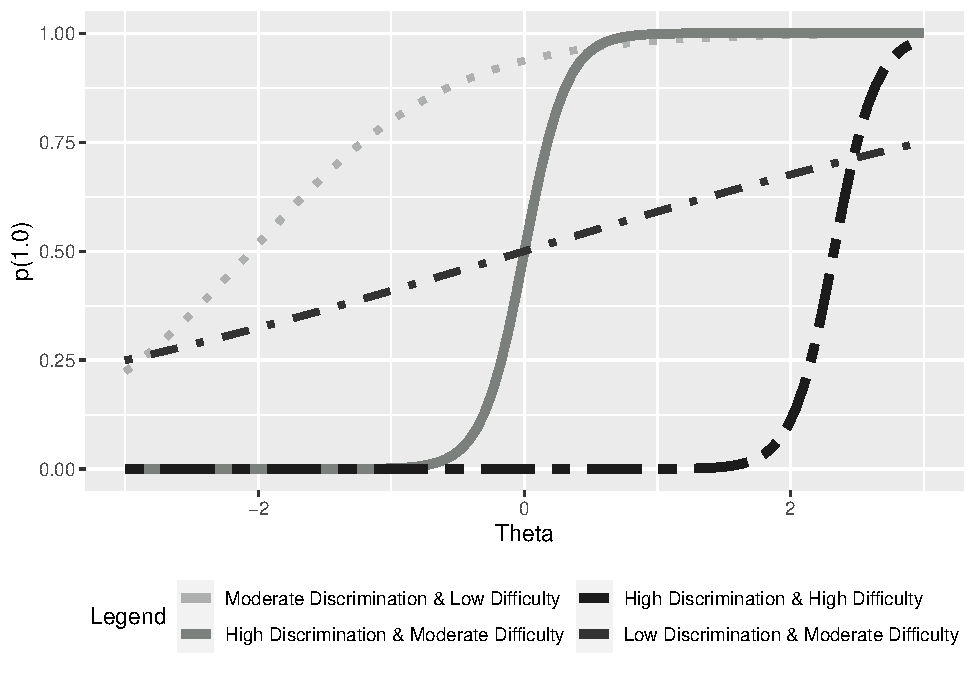
\includegraphics[width=1\linewidth,height=0.8\textheight]{ICC_project_files/figure-latex/example-1} \caption{Item characteristic curves demonstrating differences in item difficulty and discrimination.}\label{fig:example}
\end{figure}

Item characteristic curves are frequently consulted by psychometricians as visual indicators of important attributes of assessment items - most commonly \emph{difficulty} and \emph{discrimination}. Within these visual presentations the x-axis ranges along ``trait'' levels (by convention typically denoted with the greek \(\theta\)), whereas the y-axis displays probabilities of responding to the item within a given response category. In the context of true tests, the response categories are binary\footnote{With exception (see, for example, Masters, 1982; Muraki, 1997).}, and the y-axis probability reflects the likelihood of a ``correct'' response\footnote{Because the historical convention in test response is to code a correct response as ``1'' and an incorrect response as ``0'', the y-axis is commonly denoted as ``\emph{p}(1)'' or ``\emph{p}(1.0)''.}. Assessment specialists who consult ICC's usually do so from within the psychometric framework of either Item Response Theory (IRT) or Rasch modeling. These frameworks estimate the parameters necessary to plot the visual functions. Rasch models only estimate difficulty, and assume that differences in discrimination represent flaws in measurement. The IRT 2 parameter logistic model (2PL), however, estimates item discrimination in addition to item difficulty.

When interpreting an ICC, the observer extracts the relationship between a respondent's trait level and the expectation of answering the item correctly. If the curve transitions from low to high likelihood at a location toward the lower end of the trait (e.g., ``left'' on the plotting surface), this indicates that it is relatively easy to answer the item correctly. Stated in the parlance of IRT or Rasch traditions, it does not take much \(\theta\) to have a high likelihood of answering correctly. On the contrary, if the growth in the curve occurs primarily at higher trait levels, this indicates that the item is relatively more difficult. Through the lens of IRT, if discrimination is modeled and the curve is sharp (e.g., strongly vertical), this indicates high discrimination; if it is flatter, that is an indication of poorer discrimination (see Figure \ref{fig:example} for some exemplar ICCs).

Item difficulty (the IRT \emph{b}-parameter) is scaled to the trait level associated with a 50\% likelihood of correct response (e.g., it is scaled to \(\theta\)). Item discrimination (the \emph{a}-parameter) reflects the degree to which an item differentiates across individuals who are located relatively lower or higher on the trait and is scaled to the slope of the ICC function at the same 50\% likelihood of correct response location\footnote{Within the 2PL. If more item characteristics are modeled, the \emph{a}-parameter may be estimated at a different function location. \(\leftarrow\) Diego check this (look into \emph{a}-paramter scaling for the 3PL; should be halfway between lower and upper asymptotes but I'm not 100\% sure).}. From a Classical Test Theory (CTT) orientation, item difficulty is most commonly represented by the percent of individuals answering the item correctly (also referred to as a \emph{p}-value). Item discrimination can be conveyed via a few different CTT indices, but the most commonly calculated and consulted contemporary index is the corrected item-total correlation.

Assessment specialists who calculate these CTT item indices don't, by tradition, attempt to represent them visually, as is common in IRT and Rasch applications. However, ICC's based on CTT indices could possibly provide snapshot psychometric information as valuable as those conveyed by IRT- or Rasch-derived item parameters. The largest obstacle to psychometricians deeming CTT-derived visuals to be of value is likely tied to the concept of invariance, which refers to IRT parameter independence across item and person estimates. However, this property is often overstated, as invariance is only attained with perfect model-data fit (which never occurs), and is also only true after being subjected to linear transformation - commonly across samples (Rupp \& Zumbo, 2006). Additionally, several comparative investigations have noted commonality between IRT and CTT difficulty and discrimination estimates as well as relative stability of CTT estimates when samples are large and/or judisciously constructed.

\hypertarget{ctt-and-irt-comparability-investigations}{%
\subsection{CTT and IRT Comparability Investigations}\label{ctt-and-irt-comparability-investigations}}

Fan (1998) examined associations between CTT item statistics and the parameters derived from the three most popular IRT models (the 1-, 2-, and 3-parameter logistic). Correlations were very high for difficulty estimates - generally between .80 and .90. As for item discrimination, correlations were \emph{moderate} to high, with only a few being very low\footnote{And in fact, as is presented below, the relationship between the IRT and CTT discrimination indices is non-linear. The Pearson's product moment correlation is therefore \emph{not} the most appropriate index to capture the extent of the magnitude of this relationship.}. Fan (1998) also investigated index invariance for all models. In theory, the major advantage of IRT models over CTT is that the latter has an interdependency between the item and person statistics, whereas under ideal circumstances IRT parameters have no such dependency. For example, within CTT examinations, the average item difficulty is equivalent to the average person score - these indices are merely reflective of averages computed across rows or columns. What Fan (1998) reported in his study, however, did not support the purported invariant advantage of IRT parameters over CTT indices. Both CTT-derived item difficulty and discrimination indices exhibited similar levels of invariance to the IRT-derived parameters, suggesting a high level of comparability.

There have also been suggestions that the invariance property be conceptualized as a graded continuum instead of a categorical (invariant or non-invariant) population property (Hambleton et al., 1991; Rupp \& Zumbo, 2004). Estimates of IRT parameters across different calibration runs can be looked at for evidence of a possible lack of invariance. This doesn't happen with CTT item parameters, since they will always be sample-dependent. This dependency, however, is greatly influenced by the sampling strategy. Large scale data, truly random sampling, and large range items could give comparable CTT item and person statistics across testing populations and occasions (Kulas et al., 2017). Additionally, there are several empirical investigations that note high levels of ``invariance'' of CTT estimates, in some cases surpassing IRT item estimates in their capacity to have cross-sample stability (Fan, 1998; Macdonald \& Paunonen, 2002).

(Fan, 1998) in fact summarizes that the IRT and CTT frameworks ``\ldots produce very similar item and person statistics'' (p.379). Hambleton and Jones (1993) state that ``no study provides enough empirical evidence on the extent of disparity between the two frameworks and the superiority of IRT over CTT despite the theoretical differences''.

\hypertarget{relationships-between-irt-and-ctt-indices}{%
\subsection{Relationship(s) between IRT and CTT Indices}\label{relationships-between-irt-and-ctt-indices}}

Lord (1980) provided a conceptual function to describe the approximate nonlinear relationship between the IRT \emph{a}-parameter and the CTT discrimination index\footnote{Lord (1980)'s CTT discrimination index is actually the item-test biserial correlation as opposed to the contemporarily more popular \emph{corrected} item-total \emph{point-biserial} correlation. The revision (equation 2) utilizes the corrected item-total point-biserial correlation.}:

\begin{equation}
a_i\cong \frac{r_i}{\sqrt{1-r_i^2}}
\end{equation}

This formula wasn't intended for practical purposes but rather was presented as an attempt to help assessment specialists who were more familiar with CTT procedures to better understand the IRT discrimination parameter. In an effort to move from the conceptual to a more practical application, Kulas et al. (2017) proposed a modification focused on minimizing predicted residuals (either \(a_i\) or \(r_i\), with \(r_i\) being the \emph{corrected} item-total \emph{point-biserial} correlation).

The Kulas et al. (2017) investigations identified systematically predictive differences in the relationship between \(a_i\) and \(r_i\) across items with differing item difficulty values, so their alteration to Lord (1980)'s formula included a moderating effect for item difficulty (this formulaic specification is also retained in the current presentation):

\begin{equation}
\hat{a_i}\cong[(.51 + .02z_g + .3z_g^2)r]+[(.57 - .009z_g + .19z_g^2)\frac{e^r-e^{-r}}{e-e^r}]
\end{equation}

Where \(g\) is the absolute deviation from 50\% responding an item correctly and 50\% responding incorrectly (e.g., a ``\emph{p}-value'' of .5). \(z_g\) is the standard normal deviate associated with \(g\). This transformation of the common \emph{p}-value was recommended by Kulas et al. (2017) in order to scale the CTT index along a (closer to) interval-level metric more directly analogous to the IRT \emph{b}-parameter.

\hypertarget{study-1}{%
\section{Study 1}\label{study-1}}

The ultimate goal of the current project is to generate CTT-derived ICCs. As a comparative standard, however, we would also like to compare these newer CTT-derived ICCs against the IRT-derived ICC standards. These comparisons are only feasible if the CTT statistic can be reasonably expressed on the IRT parameter metric (or vice versa). Although ogives could be specified directly from the CTT-derived statistics, we made a procedural decision to retain the IRT 2PL as our functional definition for both IRT and CTT ogive specification:

\begin{equation}
P(\Theta)=\frac{1}{1+e^{-1.7a(\Theta-b)}}
\end{equation}

Kulas et al. (2017) provided a scaling of the CTT corrected item-total correlation to the metric of the IRT \emph{a}-parameter, facilitating a ``pseudo''=a approximate.\footnote{We noted throughout our investigations that the ``pseudo'' a was systematically underpredicting the actual IRT a-parameter, so we ran regressions to further modify the ``pseudo''-a scaling from the original Kulas et al. (2017) formula. Our regression modification added a further slope coefficient of 1.71633 which resulted in a more accurate rescaling of the CTT corrected item-total correlation.} Fan (1998) demonstrated strong associations between the CTT \emph{p}-value and IRT \emph{b}-parameter, but did not attempt a scaling linkage. Study 1 is therefore focused on the development of a linking equation such that the CTT \emph{p}-value may be approximated along the IRT \emph{b}-parameter metric.

\hypertarget{method}{%
\section{Method}\label{method}}

\begin{figure}
\centering
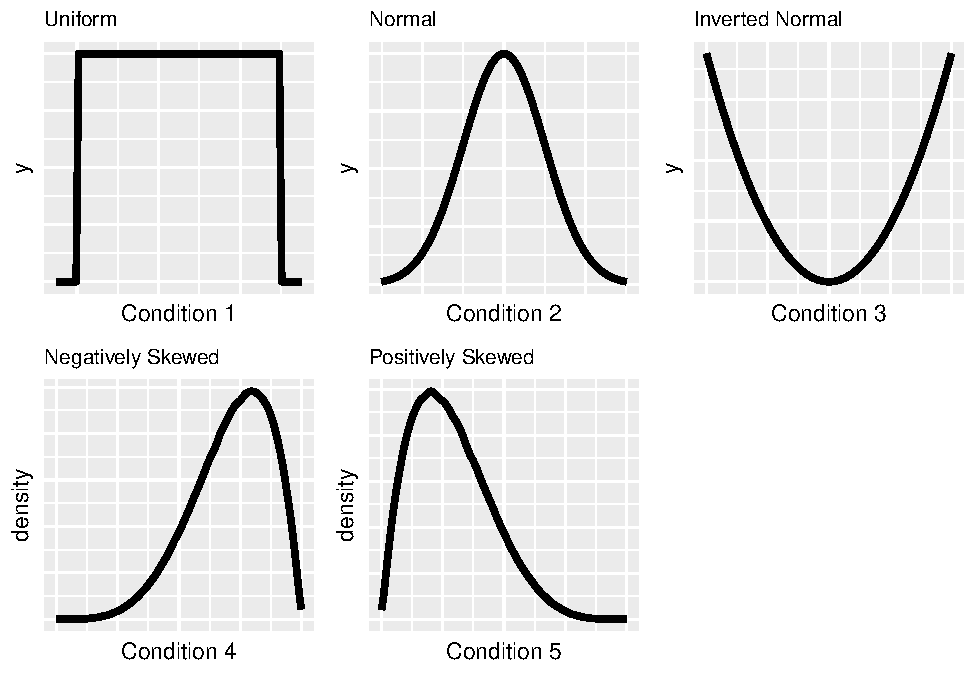
\includegraphics{ICC_project_files/figure-latex/simulatedgraphs-1.pdf}
\caption{\label{fig:simulatedgraphs}Shape of prescribed distributions of \emph{p}-values across Study 1 conditions.}
\end{figure}

\hypertarget{procedure-and-methods}{%
\subsection{Procedure and methods}\label{procedure-and-methods}}

\begin{enumerate}
\def\labelenumi{\arabic{enumi}.}
\tightlist
\item
  Purpose: Getting a p-value \(\rightarrow\) b-parameter linking equation {[}\(\checkmark\){]}
\item
  Five different distributions of p-values (simulated data) {[}\(\checkmark\){]}
\item
  10,000 runs each simulation (100 items, 10,000 ``people'' each) {[}\(\checkmark\){]}\\
\item
  Scrub extreme values (p-values essentially 0 and 1 need to be deleted) {[}\(\checkmark\){]}
\item
  Moderated regression to look for differences across p-value distribution {[} {]}
\item
  Tada! {[} {]}
\end{enumerate}

We simulated datasets comprised of binary item responses. The 10,000 individual simulated datasets primarily differed in \emph{distributions of item difficulty} while keeping the numbers of items (\emph{k}=100) and ``respondents'' (\emph{n}=10,000) equivalent. The first controlled distributional form was uniform, with \emph{p}-values ranging from low (approaching 0) to high (approaching 1) {[}NEED APPROXIMATE OR SPECIFIED VALUES HERE - NEED TO BE MORE SPECIFIC; DIEGO FILL IN{]} at roughly equal levels of frequency. The second distribution was effectively normal with \emph{p}-values centered around 0.5. The third distribution was an inverted normal distribution also centered around 0.5. The fourth distribution was a negatively skewed distribution of \emph{p}-values, and the fifth was positively skewed. Figure \ref{fig:simulatedgraphs} provides a visual representation of the \emph{p}-value distributional forms that were prescribed across our simulations.
For each simulation, we estimated CTT \emph{p}-values and corrected item-total correlations via the \texttt{psych} package (William Revelle, 2023). The 2PL was also applied via the \texttt{mirt} package (Chalmers, 2012), and \emph{a} and \emph{b} parameters were estimated. Separate and overall regressions were applied to predict the IRT \emph{b} parameter from the \emph{p}-value derived \(z_g\) statistic.

\hypertarget{results}{%
\subsection{Results}\label{results}}

Across all five conditions, simulated distributions exhibited an average empirical \emph{a}-estimate of ?? (sd = ??) and average empirical \emph{b}-estimate of ?? (sd = ??).

Overall, the average slope was \emph{r slope} and the average intercept \emph{r intercept}. \(\leftarrow\) Make sure this formula is in study 2

put in moderated regression results as well as \(\Delta R^2\) across hierarchical regressions (interaction terms added step 2).

\hypertarget{study-2---evaluating-the-comparability-of-irt-and-ctt-iccs}{%
\section{Study 2 - Evaluating the Comparability of IRT and CTT ICC's}\label{study-2---evaluating-the-comparability-of-irt-and-ctt-iccs}}

The purpose of study 2 is to simulate test data and generate ICC's based on the IRT model. Then we compare that to our CTT estimates and look at the differences. We hypothesize that on average there won't be a big difference between the curves plotted with either methodology.

\begin{enumerate}
\def\labelenumi{\arabic{enumi}.}
\tightlist
\item
  Use regression equation from Study 1
\item
  Winsteps and ETS data
\item
  Compute DIF and report results
\end{enumerate}

\hypertarget{procedure-and-materials}{%
\subsubsection{Procedure and materials}\label{procedure-and-materials}}

We used a simulated dataset and two real-world datasets. The real-world dataset represented responses from 10,000 TOEFL iBT test-takers. This test measures all four academic English skills: reading (k=39), listening (k=40), and speaking (k=35). The two TOEFL ITP datasets come from two test forms and include item-level scores. Each form includes data from 10,000 examinees, and the examinee populations for the two forms do not overlap.

The mirt package (Chalmers, 2012) was used to compute and plot the IRT statistics. To quantify the degree of difference between the two curves, the Area Between Curves was computed using Alfaro et al. (2009)'s package. Figure \ref{fig:plotting} presents some example ICCs exhibiting small, moderate, and relatively large levels of DIF. Here, the blue curves were plotted using 2PL IRT parameters (a and b), while the red curves were plotted using CTT parameters (p-values and corrected item-total correlations, re-scaling and modifying them with Kulas et al. (2017) formulas).

\hypertarget{plotting-space}{%
\subsubsection{Plotting space}\label{plotting-space}}

We need a figure with three different ICCs: 1) small DIF, 2) moderate DIF, and 3) large DIF. For each simulated scenario, compute and report our DIF index so the reader understand what the number refers to (e.g., area as defined by plotting space).

\hypertarget{results-1}{%
\subsection{Results}\label{results-1}}

\begin{verbatim}
## Iteration: 1, Log-Lik: -489327.130, Max-Change: 1.17416Iteration: 2, Log-Lik: -469788.775, Max-Change: 0.37620Iteration: 3, Log-Lik: -468634.883, Max-Change: 0.20397Iteration: 4, Log-Lik: -467874.535, Max-Change: 0.17494Iteration: 5, Log-Lik: -467193.953, Max-Change: 0.14652Iteration: 6, Log-Lik: -466779.316, Max-Change: 0.18203Iteration: 7, Log-Lik: -466457.865, Max-Change: 0.12679Iteration: 8, Log-Lik: -466185.053, Max-Change: 0.21246Iteration: 9, Log-Lik: -465979.616, Max-Change: 0.12874Iteration: 10, Log-Lik: -465781.416, Max-Change: 0.16724Iteration: 11, Log-Lik: -465638.502, Max-Change: 0.17554Iteration: 12, Log-Lik: -465518.271, Max-Change: 0.16207Iteration: 13, Log-Lik: -465417.134, Max-Change: 0.15501Iteration: 14, Log-Lik: -465328.505, Max-Change: 0.20965Iteration: 15, Log-Lik: -465241.958, Max-Change: 0.21315Iteration: 16, Log-Lik: -465146.021, Max-Change: 0.14391Iteration: 17, Log-Lik: -465077.478, Max-Change: 0.15163Iteration: 18, Log-Lik: -465023.895, Max-Change: 0.14181Iteration: 19, Log-Lik: -464976.919, Max-Change: 0.13242Iteration: 20, Log-Lik: -464936.454, Max-Change: 0.11597Iteration: 21, Log-Lik: -464899.856, Max-Change: 0.12111Iteration: 22, Log-Lik: -464868.518, Max-Change: 0.08595Iteration: 23, Log-Lik: -464839.042, Max-Change: 0.14069Iteration: 24, Log-Lik: -464814.698, Max-Change: 0.10092Iteration: 25, Log-Lik: -464790.048, Max-Change: 0.16151Iteration: 26, Log-Lik: -464770.315, Max-Change: 0.10485Iteration: 27, Log-Lik: -464747.307, Max-Change: 0.16839Iteration: 28, Log-Lik: -464726.958, Max-Change: 0.07979Iteration: 29, Log-Lik: -464709.290, Max-Change: 0.12572Iteration: 30, Log-Lik: -464694.857, Max-Change: 0.07725Iteration: 31, Log-Lik: -464679.665, Max-Change: 0.12508Iteration: 32, Log-Lik: -464667.254, Max-Change: 0.05857Iteration: 33, Log-Lik: -464656.652, Max-Change: 0.09708Iteration: 34, Log-Lik: -464648.280, Max-Change: 0.05723Iteration: 35, Log-Lik: -464639.185, Max-Change: 0.09532Iteration: 36, Log-Lik: -464631.961, Max-Change: 0.01845Iteration: 37, Log-Lik: -464623.509, Max-Change: 0.05459Iteration: 38, Log-Lik: -464618.882, Max-Change: 0.04734Iteration: 39, Log-Lik: -464614.333, Max-Change: 0.06414Iteration: 40, Log-Lik: -464610.914, Max-Change: 0.01408Iteration: 41, Log-Lik: -464605.874, Max-Change: 0.01440Iteration: 42, Log-Lik: -464602.042, Max-Change: 0.01456Iteration: 43, Log-Lik: -464585.903, Max-Change: 0.01272Iteration: 44, Log-Lik: -464584.728, Max-Change: 0.00939Iteration: 45, Log-Lik: -464583.720, Max-Change: 0.00854Iteration: 46, Log-Lik: -464579.421, Max-Change: 0.00306Iteration: 47, Log-Lik: -464579.117, Max-Change: 0.00424Iteration: 48, Log-Lik: -464578.855, Max-Change: 0.00372Iteration: 49, Log-Lik: -464578.002, Max-Change: 0.00373Iteration: 50, Log-Lik: -464577.832, Max-Change: 0.00259Iteration: 51, Log-Lik: -464577.678, Max-Change: 0.00358Iteration: 52, Log-Lik: -464577.499, Max-Change: 0.00147Iteration: 53, Log-Lik: -464577.426, Max-Change: 0.00162Iteration: 54, Log-Lik: -464577.374, Max-Change: 0.00129Iteration: 55, Log-Lik: -464577.237, Max-Change: 0.00253Iteration: 56, Log-Lik: -464577.173, Max-Change: 0.00118Iteration: 57, Log-Lik: -464577.126, Max-Change: 0.00135Iteration: 58, Log-Lik: -464576.972, Max-Change: 0.00128Iteration: 59, Log-Lik: -464576.925, Max-Change: 0.00130Iteration: 60, Log-Lik: -464576.887, Max-Change: 0.00115Iteration: 61, Log-Lik: -464576.697, Max-Change: 0.00108Iteration: 62, Log-Lik: -464576.675, Max-Change: 0.00068Iteration: 63, Log-Lik: -464576.654, Max-Change: 0.00074Iteration: 64, Log-Lik: -464576.546, Max-Change: 0.00060Iteration: 65, Log-Lik: -464576.539, Max-Change: 0.00020Iteration: 66, Log-Lik: -464576.534, Max-Change: 0.00019Iteration: 67, Log-Lik: -464576.509, Max-Change: 0.00142Iteration: 68, Log-Lik: -464576.490, Max-Change: 0.00035Iteration: 69, Log-Lik: -464576.486, Max-Change: 0.00017Iteration: 70, Log-Lik: -464576.476, Max-Change: 0.00096Iteration: 71, Log-Lik: -464576.460, Max-Change: 0.00025Iteration: 72, Log-Lik: -464576.457, Max-Change: 0.00019Iteration: 73, Log-Lik: -464576.445, Max-Change: 0.00091Iteration: 74, Log-Lik: -464576.431, Max-Change: 0.00032Iteration: 75, Log-Lik: -464576.428, Max-Change: 0.00017Iteration: 76, Log-Lik: -464576.420, Max-Change: 0.00086Iteration: 77, Log-Lik: -464576.408, Max-Change: 0.00025Iteration: 78, Log-Lik: -464576.405, Max-Change: 0.00082Iteration: 79, Log-Lik: -464576.391, Max-Change: 0.00020Iteration: 80, Log-Lik: -464576.388, Max-Change: 0.00079Iteration: 81, Log-Lik: -464576.378, Max-Change: 0.00016Iteration: 82, Log-Lik: -464576.378, Max-Change: 0.00015Iteration: 83, Log-Lik: -464576.375, Max-Change: 0.00076Iteration: 84, Log-Lik: -464576.366, Max-Change: 0.00074Iteration: 85, Log-Lik: -464576.340, Max-Change: 0.00106Iteration: 86, Log-Lik: -464576.329, Max-Change: 0.00033Iteration: 87, Log-Lik: -464576.327, Max-Change: 0.00009
##          F1     h2
## X1    0.698 0.4871
## X1.1  0.834 0.6955
## X1.2  0.818 0.6683
## X1.3  0.902 0.8144
## X1.4  0.705 0.4968
## X1.5  0.728 0.5303
## X0    0.774 0.5997
## X1.6  0.835 0.6965
## X1.7  0.900 0.8107
## X1.8  0.810 0.6568
## X1.9  0.722 0.5216
## X1.10 0.689 0.4741
## X1.11 0.726 0.5273
## X1.12 0.739 0.5468
## X0.1  0.444 0.1973
## X1.13 0.656 0.4309
## X1.14 0.698 0.4866
## X1.15 0.793 0.6293
## X1.16 0.779 0.6070
## X1.17 0.649 0.4216
## X1.18 0.664 0.4405
## X1.19 0.816 0.6653
## X1.20 0.347 0.1206
## X1.21 0.714 0.5094
## X1.22 0.821 0.6744
## X1.23 0.483 0.2331
## X1.24 0.735 0.5400
## X1.25 0.883 0.7803
## X1.26 0.605 0.3666
## X1.27 0.836 0.6982
## X1.28 0.891 0.7947
## X1.29 0.844 0.7115
## X1.30 0.859 0.7371
## X1.31 0.782 0.6121
## X1.32 0.270 0.0726
## X1.33 0.789 0.6225
## X1.34 0.806 0.6502
## X0.2  0.363 0.1321
## X1.35 0.618 0.3819
## X1.36 0.625 0.3903
## X0.3  0.514 0.2646
## X1.37 0.552 0.3049
## X1.38 0.900 0.8092
## X1.39 0.450 0.2027
## X0.4  0.663 0.4401
## X1.40 0.787 0.6199
## X1.41 0.703 0.4944
## X1.42 0.756 0.5717
## X1.43 0.779 0.6070
## X1.44 0.434 0.1881
## X1.45 0.777 0.6040
## X1.46 0.844 0.7121
## X1.47 0.798 0.6360
## X0.5  0.293 0.0861
## X1.48 0.491 0.2408
## X1.49 0.812 0.6593
## X1.50 0.794 0.6307
## X1.51 0.838 0.7021
## X1.52 0.665 0.4420
## X1.53 0.910 0.8275
## X1.54 0.837 0.6999
## X1.55 0.656 0.4298
## X1.56 0.613 0.3760
## X1.57 0.547 0.2997
## X1.58 0.651 0.4233
## X1.59 0.829 0.6871
## X1.60 0.494 0.2438
## X1.61 0.616 0.3793
## X1.62 0.850 0.7228
## X1.63 0.733 0.5373
## X1.64 0.772 0.5964
## X1.65 0.488 0.2386
## X1.66 0.827 0.6840
## X1.67 0.932 0.8680
## X1.68 0.601 0.3609
## X0.6  0.494 0.2443
## X1.69 0.765 0.5851
## X1.70 0.814 0.6618
## X1.71 0.866 0.7507
## X1.72 0.765 0.5859
## X1.73 0.679 0.4616
## X1.74 0.874 0.7647
## X1.75 0.826 0.6830
## X1.76 0.679 0.4611
## X1.77 0.760 0.5771
## X1.78 0.843 0.7109
## X1.79 0.858 0.7364
## X1.80 0.768 0.5903
## X1.81 0.819 0.6709
## X1.82 0.563 0.3175
## X1.83 0.816 0.6659
## X0.7  0.648 0.4194
## X1.84 0.617 0.3812
## X1.85 0.745 0.5551
## X0.8  0.824 0.6790
## X1.86 0.883 0.7805
## X1.87 0.598 0.3577
## X1.88 0.865 0.7480
## X1.89 0.789 0.6232
## X1.90 0.758 0.5753
## 
## SS loadings:  53.609 
## Proportion Var:  0.536 
## 
## Factor correlations: 
## 
##    F1
## F1  1
## Iteration: 1, Log-Lik: -238406.482, Max-Change: 0.54194Iteration: 2, Log-Lik: -235675.950, Max-Change: 0.18596Iteration: 3, Log-Lik: -235441.786, Max-Change: 0.06380Iteration: 4, Log-Lik: -235388.758, Max-Change: 0.04394Iteration: 5, Log-Lik: -235359.998, Max-Change: 0.03578Iteration: 6, Log-Lik: -235342.774, Max-Change: 0.02368Iteration: 7, Log-Lik: -235333.784, Max-Change: 0.01702Iteration: 8, Log-Lik: -235328.707, Max-Change: 0.01278Iteration: 9, Log-Lik: -235325.781, Max-Change: 0.01013Iteration: 10, Log-Lik: -235321.499, Max-Change: 0.00246Iteration: 11, Log-Lik: -235321.448, Max-Change: 0.00138Iteration: 12, Log-Lik: -235321.433, Max-Change: 0.00083Iteration: 13, Log-Lik: -235321.418, Max-Change: 0.00028Iteration: 14, Log-Lik: -235321.416, Max-Change: 0.00012Iteration: 15, Log-Lik: -235321.415, Max-Change: 0.00011Iteration: 16, Log-Lik: -235321.412, Max-Change: 0.00009
##         F1     h2
## LC1  0.687 0.4724
## LC2  0.664 0.4407
## LC3  0.584 0.3405
## LC4  0.519 0.2689
## LC5  0.668 0.4458
## LC7  0.649 0.4209
## LC8  0.703 0.4947
## LC9  0.680 0.4626
## LC10 0.559 0.3121
## LC11 0.478 0.2283
## LC13 0.714 0.5091
## LC14 0.586 0.3432
## LC15 0.593 0.3522
## LC16 0.478 0.2288
## LC17 0.288 0.0830
## LC19 0.562 0.3158
## LC20 0.623 0.3880
## LC21 0.547 0.2996
## LC22 0.597 0.3566
## LC23 0.721 0.5196
## LC25 0.523 0.2736
## LC26 0.569 0.3239
## LC27 0.582 0.3384
## LC28 0.356 0.1267
## LC29 0.667 0.4448
## LC31 0.616 0.3793
## LC32 0.466 0.2169
## LC33 0.595 0.3539
## LC34 0.382 0.1461
## LC35 0.482 0.2326
## LC36 0.361 0.1305
## LC37 0.574 0.3291
## LC38 0.592 0.3506
## LC39 0.509 0.2590
## LC40 0.218 0.0475
## LC41 0.473 0.2233
## LC47 0.294 0.0867
## LC48 0.339 0.1149
## LC49 0.535 0.2865
## LC50 0.346 0.1194
## 
## SS loadings:  12.066 
## Proportion Var:  0.302 
## 
## Factor correlations: 
## 
##    F1
## F1  1
## Iteration: 1, Log-Lik: -206119.950, Max-Change: 0.45550Iteration: 2, Log-Lik: -204703.235, Max-Change: 0.17689Iteration: 3, Log-Lik: -204543.730, Max-Change: 0.07766Iteration: 4, Log-Lik: -204488.227, Max-Change: 0.04568Iteration: 5, Log-Lik: -204462.138, Max-Change: 0.02917Iteration: 6, Log-Lik: -204449.368, Max-Change: 0.02094Iteration: 7, Log-Lik: -204442.263, Max-Change: 0.01543Iteration: 8, Log-Lik: -204438.269, Max-Change: 0.01169Iteration: 9, Log-Lik: -204435.897, Max-Change: 0.00876Iteration: 10, Log-Lik: -204432.888, Max-Change: 0.00368Iteration: 11, Log-Lik: -204432.576, Max-Change: 0.00266Iteration: 12, Log-Lik: -204432.386, Max-Change: 0.00138Iteration: 13, Log-Lik: -204432.183, Max-Change: 0.00124Iteration: 14, Log-Lik: -204432.109, Max-Change: 0.00109Iteration: 15, Log-Lik: -204432.052, Max-Change: 0.00097Iteration: 16, Log-Lik: -204431.919, Max-Change: 0.00056Iteration: 17, Log-Lik: -204431.902, Max-Change: 0.00057Iteration: 18, Log-Lik: -204431.889, Max-Change: 0.00054Iteration: 19, Log-Lik: -204431.838, Max-Change: 0.00017Iteration: 20, Log-Lik: -204431.837, Max-Change: 0.00017Iteration: 21, Log-Lik: -204431.835, Max-Change: 0.00016Iteration: 22, Log-Lik: -204431.829, Max-Change: 0.00011Iteration: 23, Log-Lik: -204431.828, Max-Change: 0.00010Iteration: 24, Log-Lik: -204431.828, Max-Change: 0.00009
##         F1    h2
## SW1  0.518 0.268
## SW2  0.485 0.235
## SW3  0.416 0.173
## SW4  0.566 0.320
## SW5  0.446 0.199
## SW6  0.535 0.286
## SW8  0.554 0.307
## SW9  0.570 0.325
## SW10 0.611 0.373
## SW11 0.680 0.463
## SW12 0.561 0.314
## SW13 0.480 0.230
## SW14 0.595 0.354
## SW16 0.615 0.378
## SW17 0.615 0.378
## SW18 0.587 0.345
## SW19 0.364 0.132
## SW20 0.702 0.493
## SW22 0.572 0.327
## SW23 0.604 0.365
## SW24 0.618 0.382
## SW25 0.493 0.244
## SW26 0.483 0.233
## SW27 0.372 0.139
## SW29 0.646 0.418
## SW30 0.700 0.491
## SW31 0.653 0.426
## SW32 0.472 0.223
## SW33 0.436 0.190
## SW34 0.474 0.225
## SW36 0.646 0.418
## SW37 0.392 0.153
## SW38 0.428 0.183
## SW39 0.560 0.314
## SW40 0.449 0.202
## 
## SS loadings:  10.507 
## Proportion Var:  0.3 
## 
## Factor correlations: 
## 
##    F1
## F1  1
## Iteration: 1, Log-Lik: -234309.847, Max-Change: 0.61142Iteration: 2, Log-Lik: -232156.052, Max-Change: 0.20782Iteration: 3, Log-Lik: -232026.525, Max-Change: 0.07799Iteration: 4, Log-Lik: -231990.922, Max-Change: 0.04750Iteration: 5, Log-Lik: -231974.699, Max-Change: 0.03042Iteration: 6, Log-Lik: -231966.726, Max-Change: 0.01805Iteration: 7, Log-Lik: -231962.294, Max-Change: 0.01248Iteration: 8, Log-Lik: -231959.742, Max-Change: 0.00946Iteration: 9, Log-Lik: -231958.240, Max-Change: 0.00709Iteration: 10, Log-Lik: -231955.977, Max-Change: 0.00232Iteration: 11, Log-Lik: -231955.835, Max-Change: 0.00152Iteration: 12, Log-Lik: -231955.732, Max-Change: 0.00142Iteration: 13, Log-Lik: -231955.401, Max-Change: 0.00094Iteration: 14, Log-Lik: -231955.390, Max-Change: 0.00065Iteration: 15, Log-Lik: -231955.381, Max-Change: 0.00055Iteration: 16, Log-Lik: -231955.351, Max-Change: 0.00016Iteration: 17, Log-Lik: -231955.349, Max-Change: 0.00013Iteration: 18, Log-Lik: -231955.348, Max-Change: 0.00013Iteration: 19, Log-Lik: -231955.344, Max-Change: 0.00010Iteration: 20, Log-Lik: -231955.343, Max-Change: 0.00008
##         F1     h2
## RD1  0.641 0.4107
## RD2  0.668 0.4465
## RD3  0.543 0.2951
## RD4  0.724 0.5246
## RD5  0.723 0.5226
## RD6  0.476 0.2269
## RD7  0.370 0.1371
## RD8  0.507 0.2570
## RD9  0.688 0.4734
## RD10 0.483 0.2331
## RD11 0.562 0.3160
## RD12 0.644 0.4151
## RD13 0.617 0.3812
## RD14 0.564 0.3177
## RD15 0.472 0.2232
## RD16 0.645 0.4163
## RD17 0.316 0.0997
## RD18 0.494 0.2440
## RD19 0.324 0.1052
## RD20 0.398 0.1586
## RD21 0.451 0.2031
## RD22 0.230 0.0531
## RD23 0.507 0.2574
## RD24 0.467 0.2179
## RD25 0.471 0.2216
## RD26 0.603 0.3637
## RD27 0.492 0.2423
## RD28 0.466 0.2169
## RD29 0.423 0.1785
## RD41 0.515 0.2655
## RD42 0.539 0.2904
## RD43 0.594 0.3531
## RD44 0.503 0.2529
## RD45 0.523 0.2738
## RD46 0.211 0.0443
## RD47 0.469 0.2197
## RD48 0.323 0.1046
## RD49 0.516 0.2664
## RD50 0.436 0.1904
## 
## SS loadings:  10.42 
## Proportion Var:  0.267 
## 
## Factor correlations: 
## 
##    F1
## F1  1
## Iteration: 1, Log-Lik: -216334.798, Max-Change: 0.72867Iteration: 2, Log-Lik: -212161.069, Max-Change: 0.35941Iteration: 3, Log-Lik: -211424.766, Max-Change: 0.18254Iteration: 4, Log-Lik: -211034.884, Max-Change: 0.13759Iteration: 5, Log-Lik: -210825.117, Max-Change: 0.10659Iteration: 6, Log-Lik: -210705.125, Max-Change: 0.07765Iteration: 7, Log-Lik: -210630.027, Max-Change: 0.06228Iteration: 8, Log-Lik: -210583.543, Max-Change: 0.04985Iteration: 9, Log-Lik: -210553.343, Max-Change: 0.04124Iteration: 10, Log-Lik: -210532.636, Max-Change: 0.03418Iteration: 11, Log-Lik: -210518.499, Max-Change: 0.02896Iteration: 12, Log-Lik: -210508.512, Max-Change: 0.02395Iteration: 13, Log-Lik: -210501.359, Max-Change: 0.02055Iteration: 14, Log-Lik: -210496.082, Max-Change: 0.01965Iteration: 15, Log-Lik: -210491.801, Max-Change: 0.01366Iteration: 16, Log-Lik: -210482.761, Max-Change: 0.00655Iteration: 17, Log-Lik: -210481.262, Max-Change: 0.00542Iteration: 18, Log-Lik: -210479.942, Max-Change: 0.00466Iteration: 19, Log-Lik: -210474.192, Max-Change: 0.00368Iteration: 20, Log-Lik: -210473.711, Max-Change: 0.00356Iteration: 21, Log-Lik: -210473.277, Max-Change: 0.00394Iteration: 22, Log-Lik: -210471.341, Max-Change: 0.00320Iteration: 23, Log-Lik: -210471.136, Max-Change: 0.00230Iteration: 24, Log-Lik: -210470.962, Max-Change: 0.00263Iteration: 25, Log-Lik: -210470.322, Max-Change: 0.00180Iteration: 26, Log-Lik: -210470.219, Max-Change: 0.00188Iteration: 27, Log-Lik: -210470.122, Max-Change: 0.00150Iteration: 28, Log-Lik: -210469.901, Max-Change: 0.00164Iteration: 29, Log-Lik: -210469.836, Max-Change: 0.00154Iteration: 30, Log-Lik: -210469.777, Max-Change: 0.00138Iteration: 31, Log-Lik: -210469.501, Max-Change: 0.00099Iteration: 32, Log-Lik: -210469.481, Max-Change: 0.00080Iteration: 33, Log-Lik: -210469.460, Max-Change: 0.00077Iteration: 34, Log-Lik: -210469.361, Max-Change: 0.00059Iteration: 35, Log-Lik: -210469.350, Max-Change: 0.00056Iteration: 36, Log-Lik: -210469.340, Max-Change: 0.00052Iteration: 37, Log-Lik: -210469.296, Max-Change: 0.00019Iteration: 38, Log-Lik: -210469.294, Max-Change: 0.00017Iteration: 39, Log-Lik: -210469.291, Max-Change: 0.00018Iteration: 40, Log-Lik: -210469.278, Max-Change: 0.00020Iteration: 41, Log-Lik: -210469.277, Max-Change: 0.00018Iteration: 42, Log-Lik: -210469.275, Max-Change: 0.00016Iteration: 43, Log-Lik: -210469.267, Max-Change: 0.00012Iteration: 44, Log-Lik: -210469.267, Max-Change: 0.00012Iteration: 45, Log-Lik: -210469.266, Max-Change: 0.00012Iteration: 46, Log-Lik: -210469.261, Max-Change: 0.00011Iteration: 47, Log-Lik: -210469.260, Max-Change: 0.00011Iteration: 48, Log-Lik: -210469.260, Max-Change: 0.00010Iteration: 49, Log-Lik: -210469.257, Max-Change: 0.00008
##         F1    h2
## LC1  0.776 0.603
## LC2  0.717 0.514
## LC3  0.832 0.691
## LC4  0.757 0.573
## LC5  0.802 0.644
## LC7  0.784 0.615
## LC8  0.820 0.672
## LC9  0.769 0.591
## LC10 0.835 0.697
## LC11 0.783 0.613
## LC13 0.762 0.580
## LC14 0.737 0.544
## LC15 0.710 0.504
## LC16 0.762 0.581
## LC17 0.825 0.680
## LC19 0.660 0.436
## LC20 0.541 0.293
## LC21 0.700 0.490
## LC22 0.546 0.298
## LC23 0.708 0.501
## LC25 0.578 0.334
## LC26 0.488 0.238
## LC27 0.776 0.602
## LC28 0.636 0.404
## LC29 0.566 0.320
## LC31 0.734 0.539
## LC32 0.640 0.410
## LC33 0.841 0.707
## LC34 0.504 0.254
## LC35 0.514 0.264
## LC36 0.656 0.431
## LC37 0.475 0.225
## LC38 0.585 0.342
## LC39 0.442 0.196
## LC40 0.599 0.359
## LC41 0.683 0.466
## LC47 0.457 0.209
## LC48 0.519 0.269
## LC49 0.503 0.253
## LC50 0.428 0.183
## 
## SS loadings:  18.125 
## Proportion Var:  0.453 
## 
## Factor correlations: 
## 
##    F1
## F1  1
## Iteration: 1, Log-Lik: -196312.294, Max-Change: 0.63593Iteration: 2, Log-Lik: -193358.833, Max-Change: 0.22161Iteration: 3, Log-Lik: -193046.826, Max-Change: 0.11391Iteration: 4, Log-Lik: -192893.830, Max-Change: 0.08660Iteration: 5, Log-Lik: -192814.916, Max-Change: 0.08665Iteration: 6, Log-Lik: -192770.115, Max-Change: 0.04292Iteration: 7, Log-Lik: -192743.636, Max-Change: 0.03677Iteration: 8, Log-Lik: -192728.736, Max-Change: 0.03224Iteration: 9, Log-Lik: -192720.169, Max-Change: 0.02163Iteration: 10, Log-Lik: -192715.082, Max-Change: 0.01751Iteration: 11, Log-Lik: -192711.897, Max-Change: 0.01208Iteration: 12, Log-Lik: -192709.777, Max-Change: 0.00942Iteration: 13, Log-Lik: -192705.820, Max-Change: 0.00331Iteration: 14, Log-Lik: -192705.382, Max-Change: 0.00273Iteration: 15, Log-Lik: -192705.026, Max-Change: 0.00238Iteration: 16, Log-Lik: -192703.883, Max-Change: 0.00263Iteration: 17, Log-Lik: -192703.765, Max-Change: 0.00157Iteration: 18, Log-Lik: -192703.681, Max-Change: 0.00195Iteration: 19, Log-Lik: -192703.332, Max-Change: 0.00128Iteration: 20, Log-Lik: -192703.307, Max-Change: 0.00061Iteration: 21, Log-Lik: -192703.289, Max-Change: 0.00096Iteration: 22, Log-Lik: -192703.260, Max-Change: 0.00051Iteration: 23, Log-Lik: -192703.247, Max-Change: 0.00069Iteration: 24, Log-Lik: -192703.238, Max-Change: 0.00038Iteration: 25, Log-Lik: -192703.223, Max-Change: 0.00068Iteration: 26, Log-Lik: -192703.217, Max-Change: 0.00045Iteration: 27, Log-Lik: -192703.211, Max-Change: 0.00021Iteration: 28, Log-Lik: -192703.208, Max-Change: 0.00021Iteration: 29, Log-Lik: -192703.205, Max-Change: 0.00021Iteration: 30, Log-Lik: -192703.202, Max-Change: 0.00021Iteration: 31, Log-Lik: -192703.190, Max-Change: 0.00017Iteration: 32, Log-Lik: -192703.189, Max-Change: 0.00015Iteration: 33, Log-Lik: -192703.188, Max-Change: 0.00014Iteration: 34, Log-Lik: -192703.183, Max-Change: 0.00010Iteration: 35, Log-Lik: -192703.183, Max-Change: 0.00010
##         F1     h2
## SW1  0.696 0.4851
## SW2  0.373 0.1392
## SW3  0.373 0.1392
## SW4  0.604 0.3653
## SW5  0.692 0.4792
## SW6  0.746 0.5566
## SW8  0.741 0.5495
## SW9  0.672 0.4522
## SW10 0.695 0.4836
## SW11 0.598 0.3577
## SW12 0.688 0.4734
## SW13 0.519 0.2692
## SW14 0.506 0.2562
## SW16 0.608 0.3694
## SW17 0.642 0.4118
## SW18 0.425 0.1809
## SW19 0.631 0.3976
## SW20 0.542 0.2933
## SW22 0.695 0.4834
## SW23 0.786 0.6175
## SW24 0.549 0.3018
## SW25 0.693 0.4807
## SW26 0.743 0.5521
## SW27 0.608 0.3703
## SW29 0.507 0.2570
## SW30 0.700 0.4893
## SW31 0.731 0.5349
## SW32 0.741 0.5486
## SW33 0.518 0.2680
## SW34 0.529 0.2797
## SW36 0.320 0.1021
## SW37 0.498 0.2482
## SW38 0.580 0.3364
## SW39 0.601 0.3616
## SW40 0.271 0.0736
## 
## SS loadings:  12.964 
## Proportion Var:  0.37 
## 
## Factor correlations: 
## 
##    F1
## F1  1
## Iteration: 1, Log-Lik: -227538.254, Max-Change: 0.55498Iteration: 2, Log-Lik: -225587.388, Max-Change: 0.20922Iteration: 3, Log-Lik: -225367.717, Max-Change: 0.09237Iteration: 4, Log-Lik: -225275.357, Max-Change: 0.06432Iteration: 5, Log-Lik: -225223.926, Max-Change: 0.05332Iteration: 6, Log-Lik: -225195.363, Max-Change: 0.03729Iteration: 7, Log-Lik: -225179.864, Max-Change: 0.03180Iteration: 8, Log-Lik: -225170.798, Max-Change: 0.02119Iteration: 9, Log-Lik: -225165.435, Max-Change: 0.01545Iteration: 10, Log-Lik: -225162.082, Max-Change: 0.01182Iteration: 11, Log-Lik: -225159.917, Max-Change: 0.00930Iteration: 12, Log-Lik: -225158.499, Max-Change: 0.00706Iteration: 13, Log-Lik: -225155.717, Max-Change: 0.00224Iteration: 14, Log-Lik: -225155.491, Max-Change: 0.00213Iteration: 15, Log-Lik: -225155.304, Max-Change: 0.00198Iteration: 16, Log-Lik: -225154.586, Max-Change: 0.00143Iteration: 17, Log-Lik: -225154.549, Max-Change: 0.00106Iteration: 18, Log-Lik: -225154.517, Max-Change: 0.00103Iteration: 19, Log-Lik: -225154.383, Max-Change: 0.00049Iteration: 20, Log-Lik: -225154.374, Max-Change: 0.00040Iteration: 21, Log-Lik: -225154.368, Max-Change: 0.00024Iteration: 22, Log-Lik: -225154.359, Max-Change: 0.00025Iteration: 23, Log-Lik: -225154.356, Max-Change: 0.00023Iteration: 24, Log-Lik: -225154.353, Max-Change: 0.00022Iteration: 25, Log-Lik: -225154.340, Max-Change: 0.00015Iteration: 26, Log-Lik: -225154.339, Max-Change: 0.00014Iteration: 27, Log-Lik: -225154.338, Max-Change: 0.00014Iteration: 28, Log-Lik: -225154.333, Max-Change: 0.00010Iteration: 29, Log-Lik: -225154.333, Max-Change: 0.00010
##         F1    h2
## RD1  0.639 0.408
## RD2  0.482 0.233
## RD3  0.594 0.352
## RD4  0.715 0.512
## RD5  0.626 0.392
## RD6  0.445 0.198
## RD7  0.509 0.259
## RD8  0.591 0.349
## RD9  0.464 0.215
## RD10 0.642 0.413
## RD22 0.523 0.273
## RD23 0.504 0.254
## RD24 0.237 0.056
## RD25 0.650 0.422
## RD26 0.604 0.364
## RD27 0.537 0.288
## RD28 0.671 0.450
## RD29 0.561 0.314
## RD30 0.543 0.295
## RD31 0.423 0.179
## RD32 0.487 0.237
## RD33 0.674 0.454
## RD34 0.685 0.469
## RD35 0.568 0.322
## RD36 0.645 0.416
## RD37 0.574 0.329
## RD38 0.666 0.444
## RD39 0.577 0.333
## RD40 0.375 0.140
## RD41 0.757 0.573
## RD42 0.476 0.226
## RD43 0.571 0.326
## RD44 0.604 0.365
## RD45 0.556 0.310
## RD46 0.666 0.443
## RD47 0.395 0.156
## RD48 0.511 0.262
## RD49 0.468 0.219
## RD50 0.661 0.437
## 
## SS loadings:  12.69 
## Proportion Var:  0.325 
## 
## Factor correlations: 
## 
##    F1
## F1  1
\end{verbatim}

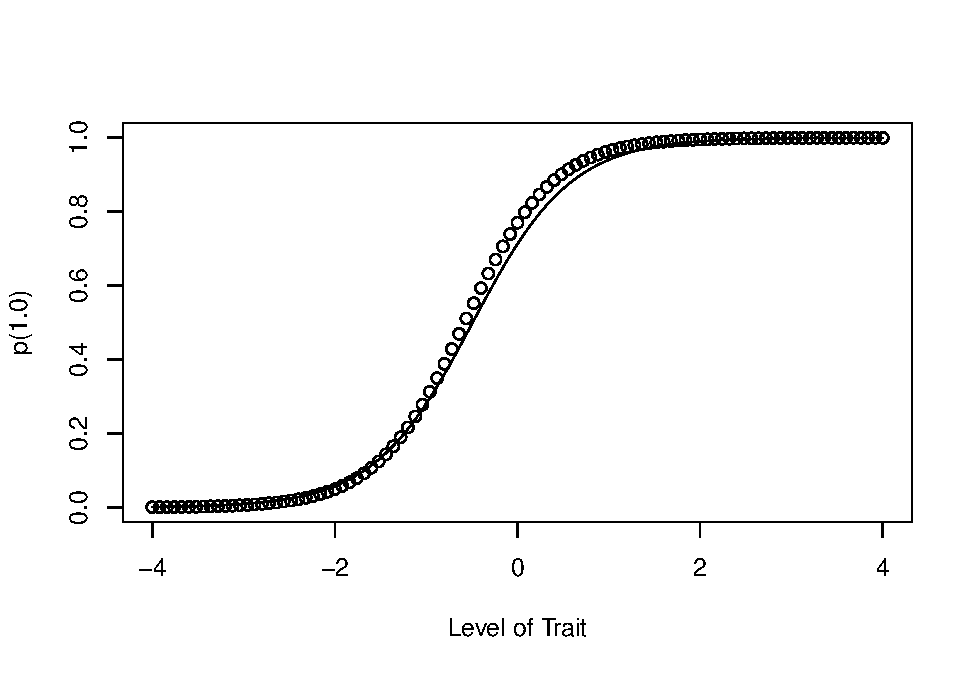
\includegraphics{ICC_project_files/figure-latex/generalrecodes-1.pdf}

We used R (Version 4.2.3; R Core Team, 2023) and the R-packages \emph{ape} (Version 5.7.1; Paradis \& Schliep, 2019), \emph{descr} (Version 1.1.7; Dirk Enzmann et al., 2023), \emph{dplyr} (Version 1.1.1; Wickham, François, et al., 2023), \emph{forcats} (Version 1.0.0; Wickham, 2023), \emph{geiger} (Version 2.0.11; Alfaro et al., 2009; Eastman et al., 2011; Harmon et al., 2008; Pennell et al., 2014; Slater et al., 2012), \emph{ggplot2} (Version 3.4.2; Wickham, 2016), \emph{gridExtra} (Version 2.3; Auguie, 2017), \emph{lattice} (Version 0.21.8; Sarkar, 2008; Sarkar \& Andrews, 2022), \emph{latticeExtra} (Version 0.6.30; Sarkar \& Andrews, 2022), \emph{lubridate} (Version 1.9.2; Grolemund \& Wickham, 2011), \emph{maps} (Version 3.4.1; Richard A. Becker et al., 2022), \emph{mirt} (Version 1.39; Chalmers, 2012), \emph{papaja} (Version 0.1.1; Aust \& Barth, 2022), \emph{phytools} (Version 1.9.16; Revell, 2012), \emph{psych} (Version 2.3.6; William Revelle, 2023), \emph{purrr} (Version 1.0.1; Wickham \& Henry, 2023), \emph{readr} (Version 2.1.4; Wickham, Hester, et al., 2023), \emph{readxl} (Version 1.4.2; Wickham \& Bryan, 2023), \emph{reticulate} (Version 1.30; Ushey et al., 2023), \emph{scales} (Version 1.2.1; Wickham \& Seidel, 2022), \emph{stringr} (Version 1.5.0; Wickham, 2022), \emph{tibble} (Version 3.2.1; Müller \& Wickham, 2023), \emph{tidyr} (Version 1.3.0; Wickham, Vaughan, et al., 2023), \emph{tidyverse} (Version 2.0.0; Wickham et al., 2019), and \emph{tinylabels} (Version 0.2.3; Barth, 2022) for all our analyses.

The area between ICC's was calculated between CTT-derived and IRT-derived ICC's. The average difference for all 100 curves was 0.08\footnote{\emph{Note}. Did the integral of the difference between the CTT and IRT functions using the ``integrate'' function in the ``stats'' package (base R). Did a test to confirm this accurately reflects the area between curves by creating two curves, one with high discrimination and another with low discrimination, and seeing what the area between curves was using first the geiger package and then base R. Also roughly estimated by hand this diff. Base R seems to be the more accurate method.}. As we can see in Figure 4, most of the data is skewed towards the lower end, indicating that out of the 100 items, most of them have areas between the curves of less than 0.11.

For Figure 5 we plotted all the 100 ICC's that use CTT parameters, and for Figure 6 we did the same but with IRT parameters instead. Curves using both methodologies are very similar in shape and form, as we can see in the two items that we point out in each figure.

\hypertarget{real-world-data}{%
\subsection{Real-world data}\label{real-world-data}}

\hypertarget{materials}{%
\subsubsection{Materials}\label{materials}}

Item responses to the Graduate Record Examination (GRE)'s XX scale were provided to the researchers from the test publisher.

Applying the CTT-derived ICC functions to real-world data and computing the DIF with the IRT-derived ICC function, the average difference for the 328 curves was0.11.

\begin{figure}
\centering
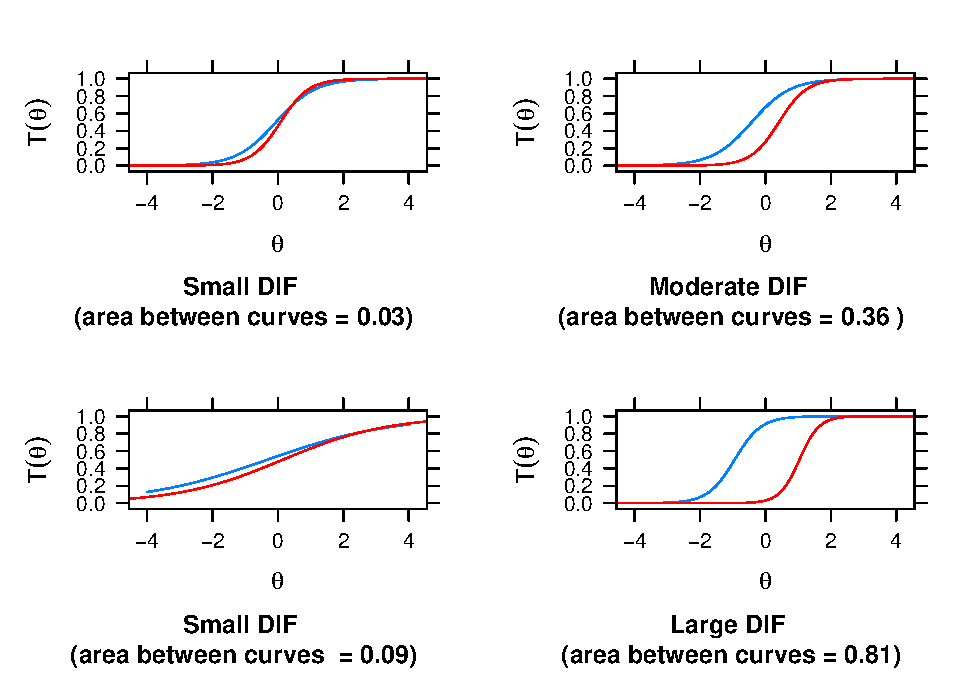
\includegraphics{ICC_project_files/figure-latex/plotting-1.pdf}
\caption{\label{fig:plotting}Four ICCs highlighting the difference between CTT and IRT-derivated ICCs at different levels of DIF.}
\end{figure}

\begin{figure}
\centering
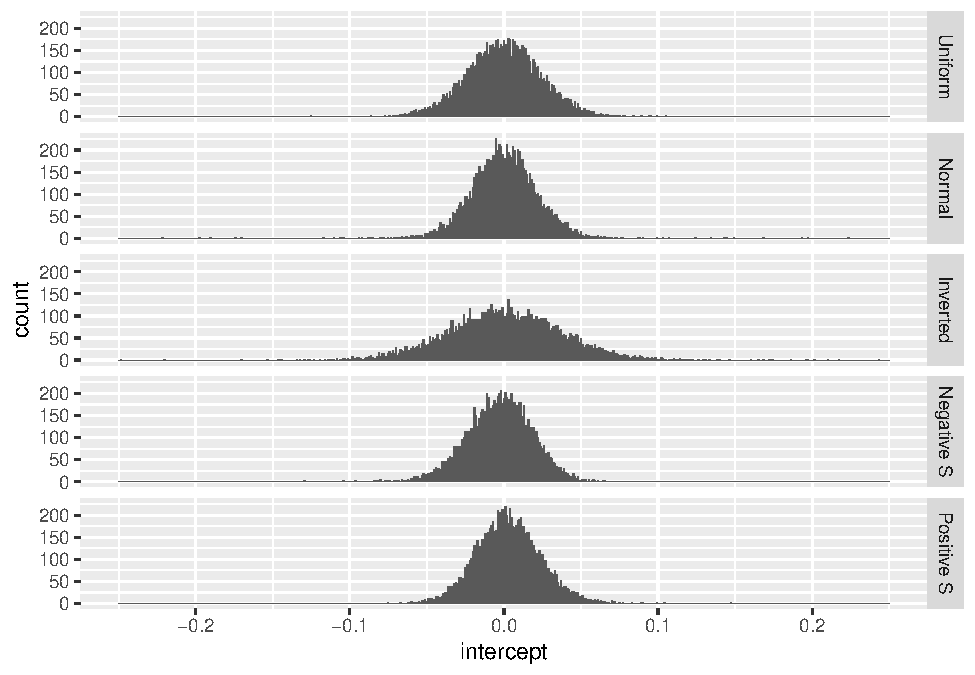
\includegraphics{ICC_project_files/figure-latex/stackedplotIntercept-1.pdf}
\caption{\label{fig:stackedplotIntercept}Individual intercept grouped by study 2 simulation.}
\end{figure}

\begin{figure}
\centering
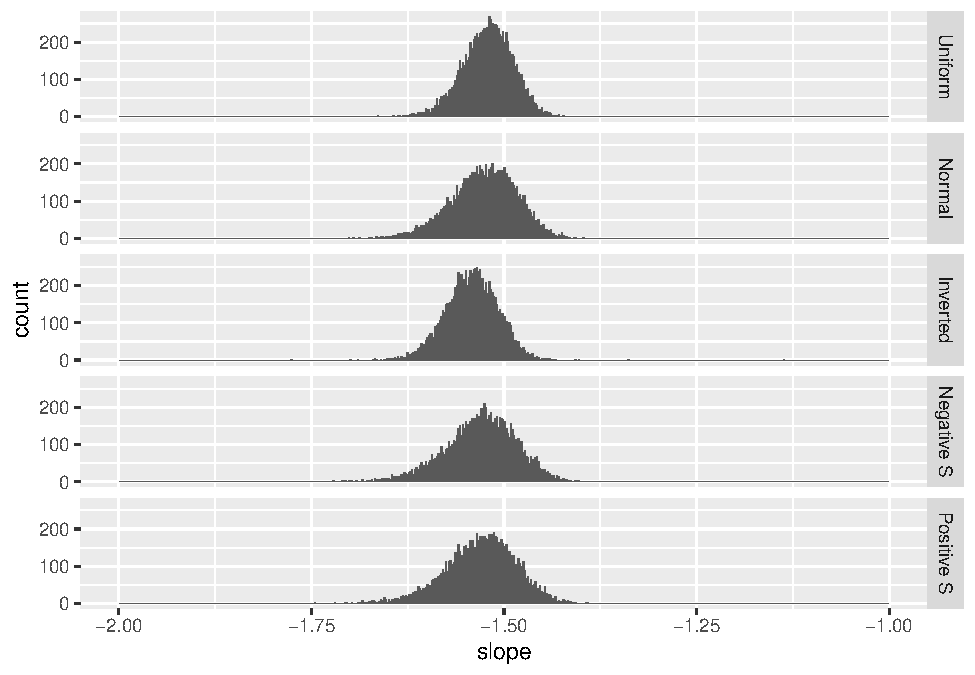
\includegraphics{ICC_project_files/figure-latex/stackeplotSlope-1.pdf}
\caption{\label{fig:stackeplotSlope}Individual slopes grouped by study 2 simulation.}
\end{figure}

\begin{figure}
\centering
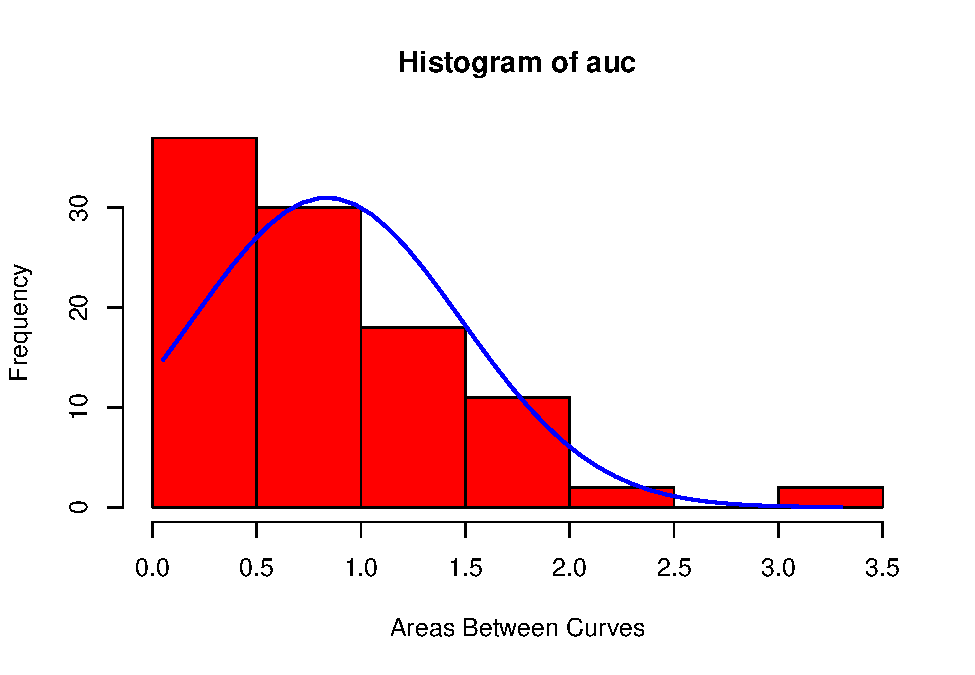
\includegraphics{ICC_project_files/figure-latex/histrogram-1.pdf}
\caption{\label{fig:histrogram}Histogram of all areas between ICCs plotted using IRT parameters vs ICCs plotted using CTT parameters.}
\end{figure}

\begin{figure}
\centering
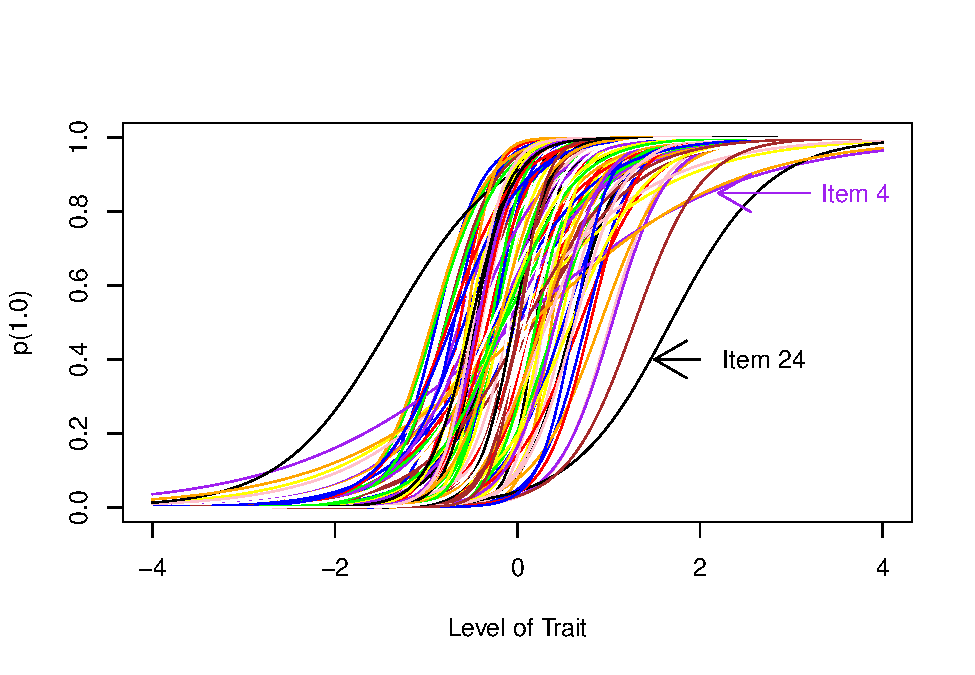
\includegraphics{ICC_project_files/figure-latex/cttcurves-1.pdf}
\caption{\label{fig:cttcurves}ICCs derived from only CTT parameters (with two noteworthy ICCs annotated).}
\end{figure}

\begin{figure}
\centering
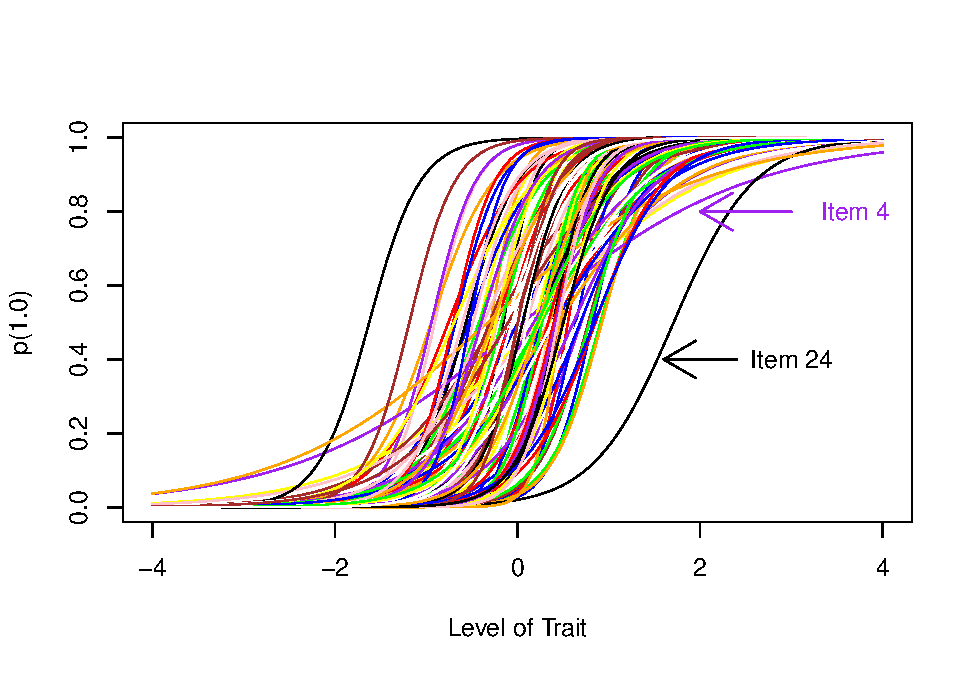
\includegraphics{ICC_project_files/figure-latex/irtcurves-1.pdf}
\caption{\label{fig:irtcurves}Typical ICCs derived from IRT parameters (same noteworthy items annotated).}
\end{figure}

\hypertarget{discussion}{%
\section{Discussion}\label{discussion}}

Important psychometric information can be gathered from ICC's, which are visual indicators typically of difficulty and discrimination. Psychometricians and other assessment specialists usually examine ICC's under the lenses of IRT and Rasch models. From a CTT orientation, item difficulty is most commonly represented by the percent of individuals answering the item correctly (also referred to as a p-value). Item discrimination can be conveyed via a few CTT indices, but the most commonly calculated and consulted index is the corrected item-total correlation. Assessment specialists who consult these CTT parameters don't typically attempt to represent them visually, as is common in IRT and Rasch applications. However, there is perhaps little reason for them not to do so, as ICC's based on CTT parameters could provide snapshot psychometric information as valuable as those gained from IRT- or Rasch-derived ICC's. Here we first propose an application of ICC's with CTT indices, then we simulated data and quantified similarities and discrepancies between the IRT- and CTT-generated ICC's. Our hypothesis was that the Area Between Curves of these different ICC's would be small. Area between curves for 100 items was 0.35 on average. This result indicates that curves plotted with either IRT or CTT parameters show little difference. The nature of both models is mostly overlapping when it comes to plotting visual representations such as ICC's. Practitioners and researchers that don't use IRT or Rasch models and instead opt to follow a CTT philosophy would benefit from having ICC's that use CTT statistics.

Of course there is always an intractability between the CTT item-difficulty index and respondent sample ability. The findings of previous comparison studies, however, point to the CTT estimates exhibiting some degree of invariance across respondent samples.

If this general idea is well-received (SIOP members would seem to represent a great barometer!) we would like to stress the CTT ICC's via further and more extensive conditions. That is, are there patterns that help explain CTT ICCs that diverge from their IRT counterparts? Although our simulations did generate a range of item difficulties and discriminations, we have not yet fully explored systematic patterns of extremely difficult/easy items as well as very poorly discriminating items. If patterns emerge, we would like to model predicted discrepancies via incorporating error bars within our visualizations. Although scaled inventory responses are more common in Psychological assessment applications, We do not believe a visual representation of the polytomous item response function (IRF) would be as practically informative, and do not foresee extensions to inventory response.

represent some promise regarding plotted ICC's using IRT and CTT parameters. Our hypothesis was that the Area Between Curves of these different ICCs would be small. Area between curves for 100 items was 0.35 on average. This result indicates that curves plotted with either IRT or CTT parameters show little difference. The nature of both models is overlapping when it comes to plotting visual representations such as ICC's. Practitioners and researchers that don't use IRT or Rasch models and instead opt to follow a CTT philosophy would benefit from having ICC's that use CTT statistics.

IRT analyses are also data hungry. These CTT-derived ICC estimates may be useful to individuals who wish to ultimately apply IRT, but are limited in\ldots{} {[}maybe not{]}

Additionally, if there is interest in this general idea we would likely publish our function as a small \texttt{R} package, perhaps to supplement the \texttt{psych} package's ``alpha'' function, which produces corrected item-total correlations as well as p-values within the same output table (e.g., the ``input'' data is already available in tabular format).

\newpage

\hypertarget{references}{%
\section{References}\label{references}}

\begingroup
\setlength{\parindent}{-0.5in}
\setlength{\leftskip}{0.5in}

\hypertarget{refs}{}
\begin{CSLReferences}{1}{0}
\leavevmode\vadjust pre{\hypertarget{ref-R-geiger_a}{}}%
Alfaro, M. E., Santini, F., Brock, C., Alamillo, H., Dornburg, A., Rabosky, D. L., Carnevale, G., \& Harmon, L. J. (2009). Nine exceptional radiations plus high turnover explain species diversity in jawed vertebrates. \emph{PNAS}, \emph{106}, 13410--13414. \url{https://doi.org/10.1073/pnas.0811087106}

\leavevmode\vadjust pre{\hypertarget{ref-R-gridExtra}{}}%
Auguie, B. (2017). \emph{gridExtra: Miscellaneous functions for "grid" graphics}. \url{https://CRAN.R-project.org/package=gridExtra}

\leavevmode\vadjust pre{\hypertarget{ref-R-papaja}{}}%
Aust, F., \& Barth, M. (2022). \emph{{papaja}: {Prepare} reproducible {APA} journal articles with {R Markdown}}. \url{https://github.com/crsh/papaja}

\leavevmode\vadjust pre{\hypertarget{ref-R-tinylabels}{}}%
Barth, M. (2022). \emph{{tinylabels}: Lightweight variable labels}. \url{https://cran.r-project.org/package=tinylabels}

\leavevmode\vadjust pre{\hypertarget{ref-R-mirt}{}}%
Chalmers, R. P. (2012). {mirt}: A multidimensional item response theory package for the {R} environment. \emph{Journal of Statistical Software}, \emph{48}(6), 1--29. \url{https://doi.org/10.18637/jss.v048.i06}

\leavevmode\vadjust pre{\hypertarget{ref-R-descr}{}}%
Dirk Enzmann, J. Aquino. I. R. source code and/or documentation written by, Schwartz, M., Jain, N., \& Kraft, S. (2023). \emph{Descr: Descriptive statistics}. \url{https://CRAN.R-project.org/package=descr}

\leavevmode\vadjust pre{\hypertarget{ref-R-geiger_b}{}}%
Eastman, J. M., Alfaro, M. E., Joyce, P., Hipp, A. L., \& Harmon, L. J. (2011). A novel comparative method for identifying shifts in the rate of character evolution on trees. \emph{Evolution}, \emph{65}, 3578--3589. \url{https://doi.org/10.1111/j.1558-5646.2011.01401.x}

\leavevmode\vadjust pre{\hypertarget{ref-fan1998item}{}}%
Fan, X. (1998). Item response theory and classical test theory: An empirical comparison of their item/person statistics. \emph{Educational and Psychological Measurement}, \emph{58}(3), 357--381.

\leavevmode\vadjust pre{\hypertarget{ref-R-lubridate}{}}%
Grolemund, G., \& Wickham, H. (2011). Dates and times made easy with {lubridate}. \emph{Journal of Statistical Software}, \emph{40}(3), 1--25. \url{https://www.jstatsoft.org/v40/i03/}

\leavevmode\vadjust pre{\hypertarget{ref-hambleton1993comparison}{}}%
Hambleton, R. K., \& Jones, R. W. (1993). Comparison of classical test theory and item response theory and their applications to test development. \emph{Educational Measurement: Issues and Practice}, \emph{12}(3), 38--47.

\leavevmode\vadjust pre{\hypertarget{ref-hambleton1991fundamentals}{}}%
Hambleton, R. K., Swaminathan, H., \& Rogers, H. J. (1991). \emph{Fundamentals of item response theory} (Vol. 2). Sage.

\leavevmode\vadjust pre{\hypertarget{ref-R-geiger_d}{}}%
Harmon, L. J., Weir, J. T., Brock, C. D., Glor, R. E., \& Challenger, W. (2008). GEIGER: Investigating evolutionary radiations. \emph{Bioinformatics}, \emph{24}, 129--131. \url{https://doi.org/10.1093/bioinformatics/btm538}

\leavevmode\vadjust pre{\hypertarget{ref-kulas2017approximate}{}}%
Kulas, J. T., Smith, J. A., \& Xu, H. (2017). Approximate functional relationship between IRT and CTT item discrimination indices: A simulation, validation, and practical extension of {Lord's} (1980) formula. \emph{Journal of Applied Measurement}, \emph{18}(4), 393--407.

\leavevmode\vadjust pre{\hypertarget{ref-lord1980applications}{}}%
Lord, F. M. (1980). \emph{Applications of IRT to practical problems}. Hillsdale: Lawrence Erlbaum Associates.

\leavevmode\vadjust pre{\hypertarget{ref-lord2012applications}{}}%
Lord, F. M. (2012). \emph{Applications of item response theory to practical testing problems}. Routledge.

\leavevmode\vadjust pre{\hypertarget{ref-macdonald2002monte}{}}%
Macdonald, P., \& Paunonen, S. V. (2002). A monte carlo comparison of item and person statistics based on item response theory versus classical test theory. \emph{Educational and Psychological Measurement}, \emph{62}(6), 921--943.

\leavevmode\vadjust pre{\hypertarget{ref-masters1982rasch}{}}%
Masters, G. N. (1982). A rasch model for partial credit scoring. \emph{Psychometrika}, \emph{47}(2), 149--174.

\leavevmode\vadjust pre{\hypertarget{ref-R-tibble}{}}%
Müller, K., \& Wickham, H. (2023). \emph{Tibble: Simple data frames}. \url{https://CRAN.R-project.org/package=tibble}

\leavevmode\vadjust pre{\hypertarget{ref-muraki1997generalized}{}}%
Muraki, E. (1997). A generalized partial credit model. In \emph{Handbook of modern item response theory} (pp. 153--164). Springer.

\leavevmode\vadjust pre{\hypertarget{ref-R-ape}{}}%
Paradis, E., \& Schliep, K. (2019). Ape 5.0: An environment for modern phylogenetics and evolutionary analyses in {R}. \emph{Bioinformatics}, \emph{35}, 526--528. \url{https://doi.org/10.1093/bioinformatics/bty633}

\leavevmode\vadjust pre{\hypertarget{ref-R-geiger_e}{}}%
Pennell, M. W., Eastman, J. M., Slater, G. J., Brown, J. W., Uyeda, J. C., Fitzjohn, R. G., Alfaro, M. E., \& Harmon, L. J. (2014). Geiger v2.0: An expanded suite of methods for fitting macroevolutionary models to phylogenetic trees. \emph{Bioinformatics}, \emph{30}, 2216--2218. \url{https://doi.org/10.1093/bioinformatics/btu181}

\leavevmode\vadjust pre{\hypertarget{ref-R-base}{}}%
R Core Team. (2023). \emph{R: A language and environment for statistical computing}. R Foundation for Statistical Computing. \url{https://www.R-project.org/}

\leavevmode\vadjust pre{\hypertarget{ref-R-phytools}{}}%
Revell, L. J. (2012). Phytools: An {R} package for phylogenetic comparative biology (and other things). \emph{Methods in Ecology and Evolution}, \emph{3}, 217--223. \url{https://doi.org/10.1111/j.2041-210X.2011.00169.x}

\leavevmode\vadjust pre{\hypertarget{ref-R-maps}{}}%
Richard A. Becker, O. S. code by, Ray Brownrigg. Enhancements by Thomas P Minka, A. R. Wilks. R. version by, \& Deckmyn., A. (2022). \emph{Maps: Draw geographical maps}. \url{https://CRAN.R-project.org/package=maps}

\leavevmode\vadjust pre{\hypertarget{ref-rupp2004note}{}}%
Rupp, A. A., \& Zumbo, B. D. (2004). A note on how to quantify and report whether IRT parameter invariance holds: When pearson correlations are not enough. \emph{Educational and Psychological Measurement}, \emph{64}(4), 588--599.

\leavevmode\vadjust pre{\hypertarget{ref-rupp2006understanding}{}}%
Rupp, A. A., \& Zumbo, B. D. (2006). Understanding parameter invariance in unidimensional IRT models. \emph{Educational and Psychological Measurement}, \emph{66}(1), 63--84.

\leavevmode\vadjust pre{\hypertarget{ref-R-lattice}{}}%
Sarkar, D. (2008). \emph{Lattice: Multivariate data visualization with r}. Springer. \url{http://lmdvr.r-forge.r-project.org}

\leavevmode\vadjust pre{\hypertarget{ref-R-latticeExtra}{}}%
Sarkar, D., \& Andrews, F. (2022). \emph{latticeExtra: Extra graphical utilities based on lattice}. \url{https://CRAN.R-project.org/package=latticeExtra}

\leavevmode\vadjust pre{\hypertarget{ref-R-geiger_c}{}}%
Slater, G. J., Harmon, L. J., Wegmann, D., Joyce, P., Revell, L. J., \& Alfaro, M. E. (2012). Fitting models of continuous trait evolution to incompletely sampled comparative data using approximate bayesian computation. \emph{Evolution}, \emph{66}, 752--762. \url{https://doi.org/10.1111/j.1558-5646.2011.01474.x}

\leavevmode\vadjust pre{\hypertarget{ref-R-reticulate}{}}%
Ushey, K., Allaire, J., \& Tang, Y. (2023). \emph{Reticulate: Interface to 'python'}. \url{https://CRAN.R-project.org/package=reticulate}

\leavevmode\vadjust pre{\hypertarget{ref-R-ggplot2}{}}%
Wickham, H. (2016). \emph{ggplot2: Elegant graphics for data analysis}. Springer-Verlag New York. \url{https://ggplot2.tidyverse.org}

\leavevmode\vadjust pre{\hypertarget{ref-R-stringr}{}}%
Wickham, H. (2022). \emph{Stringr: Simple, consistent wrappers for common string operations}. \url{https://CRAN.R-project.org/package=stringr}

\leavevmode\vadjust pre{\hypertarget{ref-R-forcats}{}}%
Wickham, H. (2023). \emph{Forcats: Tools for working with categorical variables (factors)}. \url{https://CRAN.R-project.org/package=forcats}

\leavevmode\vadjust pre{\hypertarget{ref-R-tidyverse}{}}%
Wickham, H., Averick, M., Bryan, J., Chang, W., McGowan, L. D., François, R., Grolemund, G., Hayes, A., Henry, L., Hester, J., Kuhn, M., Pedersen, T. L., Miller, E., Bache, S. M., Müller, K., Ooms, J., Robinson, D., Seidel, D. P., Spinu, V., \ldots{} Yutani, H. (2019). Welcome to the {tidyverse}. \emph{Journal of Open Source Software}, \emph{4}(43), 1686. \url{https://doi.org/10.21105/joss.01686}

\leavevmode\vadjust pre{\hypertarget{ref-R-readxl}{}}%
Wickham, H., \& Bryan, J. (2023). \emph{Readxl: Read excel files}. \url{https://CRAN.R-project.org/package=readxl}

\leavevmode\vadjust pre{\hypertarget{ref-R-dplyr}{}}%
Wickham, H., François, R., Henry, L., Müller, K., \& Vaughan, D. (2023). \emph{Dplyr: A grammar of data manipulation}. \url{https://CRAN.R-project.org/package=dplyr}

\leavevmode\vadjust pre{\hypertarget{ref-R-purrr}{}}%
Wickham, H., \& Henry, L. (2023). \emph{Purrr: Functional programming tools}. \url{https://CRAN.R-project.org/package=purrr}

\leavevmode\vadjust pre{\hypertarget{ref-R-readr}{}}%
Wickham, H., Hester, J., \& Bryan, J. (2023). \emph{Readr: Read rectangular text data}. \url{https://CRAN.R-project.org/package=readr}

\leavevmode\vadjust pre{\hypertarget{ref-R-scales}{}}%
Wickham, H., \& Seidel, D. (2022). \emph{Scales: Scale functions for visualization}. \url{https://CRAN.R-project.org/package=scales}

\leavevmode\vadjust pre{\hypertarget{ref-R-tidyr}{}}%
Wickham, H., Vaughan, D., \& Girlich, M. (2023). \emph{Tidyr: Tidy messy data}. \url{https://CRAN.R-project.org/package=tidyr}

\leavevmode\vadjust pre{\hypertarget{ref-R-psych}{}}%
William Revelle. (2023). \emph{Psych: Procedures for psychological, psychometric, and personality research}. Northwestern University. \url{https://CRAN.R-project.org/package=psych}

\end{CSLReferences}

\endgroup

\hypertarget{appendix-appendices}{%
\appendix}


\hypertarget{cut-stuff}{%
\section{Cut stuff}\label{cut-stuff}}

An adjustment to Lord (2012)'s formula giving the functional relationship between the ``non-invariant'' CTT and ``invariant'' IRT statistics becomes useful in comparing the two methodologies, despite the supposed lack of invariance from CTT. So even though here we acknowledge that invariance is a categorical IRT property, we still follow the functional modification proposed by Kulas et al. (2017), noting that having a large sample that is truly random and whose items are normally distributed and have a center at the moderate difficulty can help reduce threats to CTT ``invariance''.

\#\#NOTES
\#\#Bias might suggest that rescaled a parameters are systematically larger than z under certain simulations (or not) Variance estimates might suggest that the standard error of rescaled values is larger than those values estimated directly (or not). If differences do exist, one could then go on to articulate the conditions under which they exist (i.e., high difficulty, low difficulty, non-normal distributions of the underlying trait), etc\ldots.

\begin{quote}
\emph{Note}. Maybe do a different linking via machine learning. Try to find the linking parameters (including p-value distributional shape and location) that minimize DIF across CTT and IRT ICCs (5/27/22 after unsuccessful Friday brainstorming especially regarding simulation 3 {[}the normally distributed p-values{]})
\end{quote}

2/9/2023 Notes: Check if the a parameter is estimated at the 0.5 location of the function. Research how the a parameter is scaled.
Be more specific about the simulations. Write what we did when p-values were 0 and 1 for a column.
Check the average a and b per simulation in line 255
For graph 7 update it by stacking the results we got from our simulations with the real data from ETS

As shown by Figure 2, our plot looks very similar to that of Kulas et al. (2017) (p.8). This confirms that our formula for computing the estimated a-parameter follows the exponential relationship we can see in Kulas et al. (2017).


\end{document}
